\documentclass{article}
\usepackage{cmap}
\usepackage[utf8]{inputenc}
\usepackage[english,ukrainian]{babel}
\usepackage{graphicx}
\usepackage{geometry}
\usepackage{listings}
\usepackage{float}
\usepackage{amsmath}
\usepackage{subfig}
\geometry{
	a4paper,
	left=20mm,
	right=20mm,
	top=15mm,
	bottom=15mm,
}
\lstset{
	language=c,
	tabsize=4,
	keepspaces,
	showstringspaces=false,
}
\graphicspath{ {./pictures} }
\setlength{\parindent}{4em}

\newcommand\subject{Архітектура комп'ютера}
\newcommand\lecturer{доцент кафедри ПЗ\\Крук О.Г.}
\newcommand\teacher{доцент кафедри ПЗ\\Крук О.Г.}
\newcommand\mygroup{ПЗ-22}
\newcommand\lab{5}
\newcommand\theme{Складення та відлагодження циклічної програми мовою асемблера мікропроцесорів х86 для Windows}
\newcommand\purpose{Ознайомитись на прикладі циклічної програми з основними командами асемблера; розвинути навики складання програми з вкладеними циклами; відтранслювати і виконати в режимі відлагодження програму, складену відповідно до свого варіанту; перевірити виконання тесту}

\begin{document}
\begin{normalsize}
	\begin{titlepage}
		\thispagestyle{empty}
		\begin{center}
			\textbf{МІНІСТЕРСТВО ОСВІТИ І НАУКИ УКРАЇНИ\\
				НАЦІОНАЛЬНИЙ УНІВЕРСИТЕТ "ЛЬВІВСЬКА ПОЛІТЕХНІКА"}
		\end{center}
		\begin{flushright}
			\textbf{ІКНІ}\\
			Кафедра \textbf{ПЗ}
		\end{flushright}
		\vspace{200pt}
		\begin{center}
			\textbf{ЗВІТ}\\
			\vspace{10pt}
			до лабораторної роботи № \lab\\
			\textbf{на тему}: “\textit{\theme}”\\
			\textbf{з дисципліни}: “\subject”
		\end{center}
		\vspace{112pt}
		\begin{flushright}
			
			\textbf{Лектор}:\\
			\lecturer\\
			\vspace{28pt}
			\textbf{Виконав}:\\
			
			студент групи \mygroup\\
			Коваленко Д.М.\\
			\vspace{28pt}
			\textbf{Прийняв}:\\
			
			\teacher\\
			
			\vspace{28pt}
			«\rule{1cm}{0.15mm}» \rule{1.5cm}{0.15mm} 2022 р.\\
			$\sum$ = \rule{1cm}{0.15mm}……………\\
			
		\end{flushright}
		\vspace{\fill}
		\begin{center}
			\textbf{Львів — 2022}
		\end{center}
	\end{titlepage}
		
	\begin{description}
		\item[Тема.] \theme.
		\item[Мета.] \purpose.
	\end{description}

	\section*{Індивідуальне завдання}
	\begin{figure}[H]
		\centering
		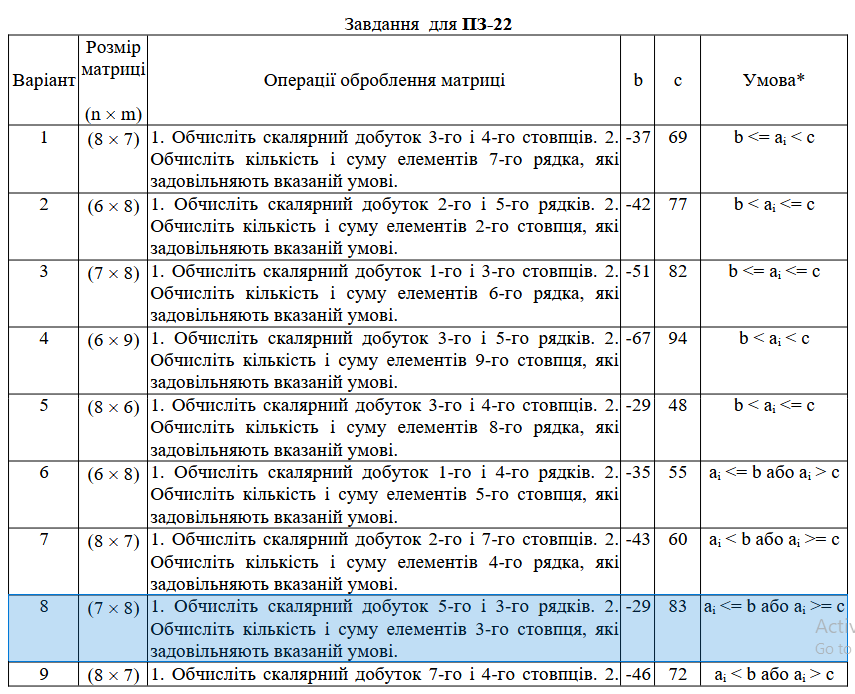
\includegraphics[scale=0.6]{v}
	\end{figure}	

	\section*{Теоретичні відомості}
	
	\section*{Хід роботи}
	\section*{Програма 1}
	\begin{figure}[H]
		\centering
		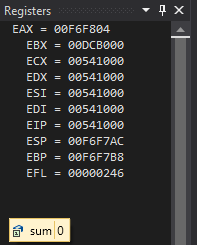
\includegraphics[scale=1]{1}
		\caption{Стан регістрів та змінної $sum$ після виконання програми}
	\end{figure}
	\begin{gather}
		17+3-51+242-113=98_{10}=62_{16}\nonumber
	\end{gather}

	\section*{Програма 2}
	\begin{gather}
		\text{3 рядок: }a= -81,-78,-82,-39,-90,-78, 24\nonumber\\
		\text{5 рядок: }b=56,-19,-86, 34,-83,-99,-31\nonumber\\
		\sum_{i=1}^{7}a_ib_i=-81\cdot56-78\cdot(-19)-82\cdot(-86)-39\cdot34-90\cdot(-83)-78\cdot(-99)+24\cdot(-31)=\nonumber\\=-4536+1482+7052-1326+7470+7722-744=17120\nonumber
	\end{gather}

	\begin{figure}[H]
		\centering
		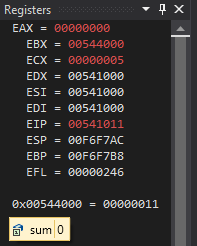
\includegraphics[scale=1]{2}
		\caption{Двовимірний масив, що необхідно було транспонувати}
	\end{figure}

	\begin{figure}[H]
		\centering
		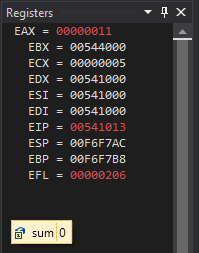
\includegraphics[scale=0.7]{3}
		\caption{Відображення транспонованого масиву у пам'яті}
	\end{figure}

	\section*{Висновки}
	
	    
\end{normalsize}
\end{document}
